

\documentclass[12pt, final]{article}

%%%%%%%%%%%%%%%%%%%%%%%%%%%%%%%%%%%%%%%%%%%%%%%
\usepackage{virgil_env} %% Import the Virgil environment
%\usepackage{multirow}
%\usepackage{fullpage}
%\usepackage{nips10submit_e}
\usepackage{afterpage}
\usepackage{cite}
\usepackage{caption}
\usepackage{subfigure}
%\usepackage{subfig}

%\usepackage{subcaption}
%\nipsfinalcopy
%\input{this_symbols.tex}  %% symbols for this paper


\usepackage[utf8]{inputenc}


\graphicspath{{./}{figs/}}
% \usepackage{booktabs,nicefrac}

\usepackage{xspace}
\usepackage{float}


\usepackage{listings} % to make pretty code


% \usepackage{tabu}% http://ctan.org/pkg/tabu

\newcommand{\dashrule}[1][black]{%
  \color{#1}\rule[\dimexpr.5ex-.2pt]{4pt}{.4pt}\xleaders\hbox{\rule{4pt}{0pt}\rule[\dimexpr.5ex-.2pt]{4pt}{.4pt}}\hfill\kern0pt%
}
\newcommand{\rulecolor}[1]{%
  \def\CT@arc@{\color{#1}}%
}

%\newcommand{\tt}[1]{{\texttt{ #1 }}}
\newcommand{\fname}[1]{ \operatorname{ #1 } }
\newcommand{\opname}[1]{ \operatorname{ #1 } }
\newcommand{\opcode}[1]{\textsc{\texttt{#1}}}


%\usepackage{authblk}
\author{Virgil Griffith}
\author{???}
\author{Vitalik Buterin}
%\affil{Ethereum Foundation}
%\affil[2]{National University of Singapore}


%%%%%%%%%%%%%%%%%%%%%%%%%%%%%%%%%%%%%%%%%%%%%%%%%%%%%%%

\bibliographystyle{plos2009}

\usepackage{mathenv}
%\usepackage[]{algorithm2e}


\title{Blockchain Resource Pricing}

%%%%%%%%%%%%%%%%%%%%%%%%%%%%%%%%%%%%%%%%%%%%%%%%%%%%%%%%%%%%%%%%%%%%%%%%%%%%%%%%%%%%%%%%%%%%%%%%

%%%%%%%%%%%%%%%%%%%%%%%%%%%%%%%%%%%%%%%%%%%%%%%%%%%%%%%%%%%%%%%%%%%%%%%%%%%%%%%%%%%%%%%%%%%%%%%%


\begin{document}

\maketitle
\vspace{-0.2in} \TODO{\today}

%{\centering {\sffamily \today} \vskip10pt }

%\vspace{-0.2in} {\centering \today } \vspace{0.1in}



%\vspace{-0.05in}
\begin{abstract}
\todo{this will be reworked at the end} 

One of the most challenging issues in blockchain protocol design is that of how to limit and price the submission of transactions that get included into the chain. Every transaction clearly confers some private benefit to its sender, but transactions also carry multiple categories of social costs to the network as a whole, including the computing power, storage space and bandwidth required by nodes to process the transaction, as well as the less easily calculable systemic risks that arise from the network becoming more centralized as the transaction load of a blockchain gets bigger and more difficult for smaller nodes to process. This results in a classic example of the ``tragedy of the commons'' problem, where transaction senders do not fully internalize the costs of their transactions, and if transactions are left unlimited and unpriced, massive overconsumption of the blockchain's resources is likely to result.

In such cases, economic theory generally dictates pricing the resources in question, and setting the price to equal the social cost that the act of consuming each resource imposes on the network. However, the heterogenous nature of the resources involved, the large portion of the social cost that exists in the form of intangible and difficult-to-value harms such as centralization risk, and the need to create an automated algorithm that can set prices in a wide range of future scenarios without human intervention all make it very difficult to set restrictions that are optimal. In this paper, we discuss tradeoffs between different approaches and strategies that can improve on the status quo on the margin.
\end{abstract}

%%%%%%%%%%%%%%%%%%%%%%%%%%%%%%%%%%%%%%%%%%%%%%%%%%%%%%%%%%%%%%%%%%%%%%%%%%
\section{Introduction and Model}
%%%%%%%%%%%%%%%%%%%%%%%%%%%%%%%%%%%%%%%%%%%%%%%%%%%%%%%%%%%%%%%%%%%%%%%%%%

A blockchain is a decentralized computer network consisting of a large number of computers that all process transactions that are uploaded to the chain. Hence, a transaction that is published to a blockchain confers some private benefit to its sender, but also confers an external social cost to the network's participants. In order to account for this social cost, and prevent abuse of the blockchain as a common pool resource, some economic mechanism for restricting what transactions get included is required. However, there are many types of mechanisms and many sets of parameters to choose from; hence, if we want to figure out what mechanism and parameters really are optimal, we need to more deeply understand how large the social cost of a transaction is and where it comes from.

The costs can be broken down in two ways. First, one can categorize by fundamental type of resource expenditure:

\begin{itemize}
\item[] \textbf{Bandwidth cost:} the cost of all nodes downloading each submitted transaction, bundling it into a block, and then rebroadcasting the transaction as part of some block.

\item[] \textbf{Computational cost:} the cost of every node verifying each transaction.

\item[] \textbf{History storage cost:} the cost of storing the transaction for all nodes that store the blockchain's history, for the time for which the history is stored (possibly infinity).

\item[] \textbf{State storage cost:} the marginal cost of the impact of the transaction on the size of the state (eg. contract code, account balances) that every node must store to be able to process further transactions.
\end{itemize}

Note that the first two costs are costs that are paid by the nodes that are online at the exact time when the transaction is included, the third cost is paid by nodes that are online at that time or in the near future, but the fourth cost must be paid by all nodes forever, unless a scheme is introduced that makes all state entries temporary.

Second, one can categorize by different types of first and second-order effects. We can understand these effects as follows. We can describe a blockchain as being a network of $n$ computers, $C_1 ... C_n$, where any transaction that gets included in the blockchain must be processed by all of the nodes that are still online in the network. Some transactions are more complex than others; each transaction has some ``weight'' $w$ that represents the quantity of resources needed to process it.

Each user $U_i$ has some direct resource cost function $R_i(W)$ representing the cost to the user of processing a given amount of weight. This cost can include electricity and bandwidth costs, marginal disk wear and tear, inconvenience from a user's other applications running more slowly, reduced battery life, and so on. For sufficiently high $w$, at some point the costs become unacceptable to any given user, at which point the user will drop offline (we assume $R_i(W)$ is flat above this point). Let $NodeCount(W)$ be the number of users still online at weight $W$. Note that different users could drop offline at different points for either of two reasons: (i) some users have a lower resource cost than others, and (ii) some users value being connected to the blockchain more than others.

There is some utility function $D(k)$ reflecting the social value of the level of decentralization achieved by having the number of online nodes, which can be translated into a function $D(W)$ of the total transaction load. There may also be some cost function $A(W)$ that reflects the increased attackability of the network as more transactions get included. We can summarize all of these costs as a combined cost function $C(W) = \sum_i R_i(W) + (A(W) - A(0)) - (D(W) - D(0))$.

The above suffices as a model of a blockchain for the purpose of this paper; we actually do not need to care about details about proof of work, proof of stake, block structure, etc, except insofar as the details of those consensus algorithms and blockchain design patterns affect $NodeCount$ and $A$, and therefore $C$.

\section{Prior Work}

In Bitcoin and Ethereum, resources are priced using a simple ``cap-and-trade'' scheme. A metric is defined for the quantity of resources (called ``weight'' or ``gas'') that a transaction consumes, and there is a protocol-defined maximum total quantity of resources that the transactions contained in a block will consume. Validators have free rein to select transactions as long as the total weight of the block is below that limit. An equilibrium is established where users attach fees to their transactions which go to the validator that includes the transaction in a block, and validators select the transactions paying the highest fee per unit weight. In Bitcoin, for example, the weight limit is a static $4 *10^6$, and weight is defined as follows:

\begin{equation}
\tt{weight(block) = 4 * len(block.nonsignature\_data) + len(block.signature\_data)}
\end{equation}

Where $len(x)$ returns the number of bytes in $x$. For technical reasons that have to do with attempting to price in history and state storage costs, the bytes in signatures of transactions are priced more cheaply than the non-signature data in transactions. In Ethereum, there is a measure called ``gas'' which incorporates the size of the block as well as the computational cost of verifying transactions and executing smart contract code. For simplicity of exposition, this can be approximated as:

\begin{equation}
\tt{weight(block) = 68 * len(block) + 3 * num\_computational\_steps\_in\_block}
\end{equation}

The gas function is in reality much more complex (See Appendix \ref{appendix:gasfunction}), but similar in spirit. There is a per-block gas limit, which validators can vote on (every validator can ``upvote'' or ``downvote'' the gas limit by a maximum of $\sim\!0.1\%$), and at the time of this writing most validators are voting for a gas limit of $\sim \! 8$ million.

A major problem with this approach is that a priori it has been difficult to determine a reasonable weight limit. Many argue that the current limit of $8$ million is far below optimal, and others disagree. The purpose of this paper will be to try to go beyond ``there must be a limit, what should it be?'' and explore a much larger space of policies that attempt to address transaction resource consumption externalities, and try to develop policies that are both closer to optimal at the present time, and more robust to changes in economic circumstances in the future, lessening the need for ``extra-protocol interventions'' such as hard forks.

\section{Pricing Resources under Uncertainty}
\label{sect:uncertainty}
Blockchain resource pricing has many parallels to regulatory responses to environmental pollution.  Particularly, although the validator of a block is compensated for publishing the transactions, the cost of that block being published is borne by \emph{all full nodes}.  This cost being borne by all full nodes is the negative externality that we wish to limit.  Both blockchains and environmental regulators use economic interventions to limit activities with negative externalities, where the negative externalities have both measurable components as well as components with high Knightian uncertainty (i.e., ``unknown unknowns'') \cite{knight1921risk}.  Many results from environmental economics \cite{barder14} are directly applicable to blockchains.

Weitzman's 1974 paper ``Prices vs Quantities'' \cite{weitzman1974prices}, outlines the tradeoffs between regulation by price (e.g., carbon taxes) versus regulation by quantity (e.g., issuing a fixed number of permits and letting them trade on the market). One important insight that Weitzman cites is that if the policymaker has perfect information about the social cost function and the demand curve for consuming the resource (a.k.a. the ``benefit function''), the two approaches are equivalent: for any desired price, one can choose an equivalent quantity-based policy by issuing exactly the number of permits equal to the equilibrium quantity that would be purchased at that price. However, when there is uncertainty about the position and shape of the cost-benefit curves, the two approaches have substantial differences.

Consider a world where the marginal social cost (negative externalities) of consuming a resource is fixed, but the marginal benefit function is rapidly decreasing. If a policymaker sets a quantity limit that is too low, then the quantity limit will intersect the marginal benefit curve at a point where the cost and benefit are much higher than the social cost, and consumers suffer very large opportunity costs from nonconsumption.  But if a policymaker instead sets a price, then the damage from a miscalculation is much lower.

If on the other hand, the \emph{private} cost of abstaining is fixed yet the marginal social cost of consumption increases rapidly, then setting a price is riskier. For example, consider a scenario where the social cost of consuming $<1,000$ resource units is acceptable, but going above 1,000 risks disastrous consequences (e.g., some ``tipping point'' theories of global warming\cite{wiki:runaway}). The marginal social cost of consuming an additional resource unit in a world where people are already consuming 1,050 resource units will be much higher than the marginal social cost in a world where people are merely consuming 900. In this case, if a policymaker anticipates a consumption of 900, and targets a tax to equal the marginal social cost at the 900 level, then the policy will be massively underpricing the additional social harm caused by additional resource consumption. On the other hand, a policymaker that simply issues 900 permits and allows them to trade on the market would see the risk mitigated.

\begin{center}
%\subfigure[]{
	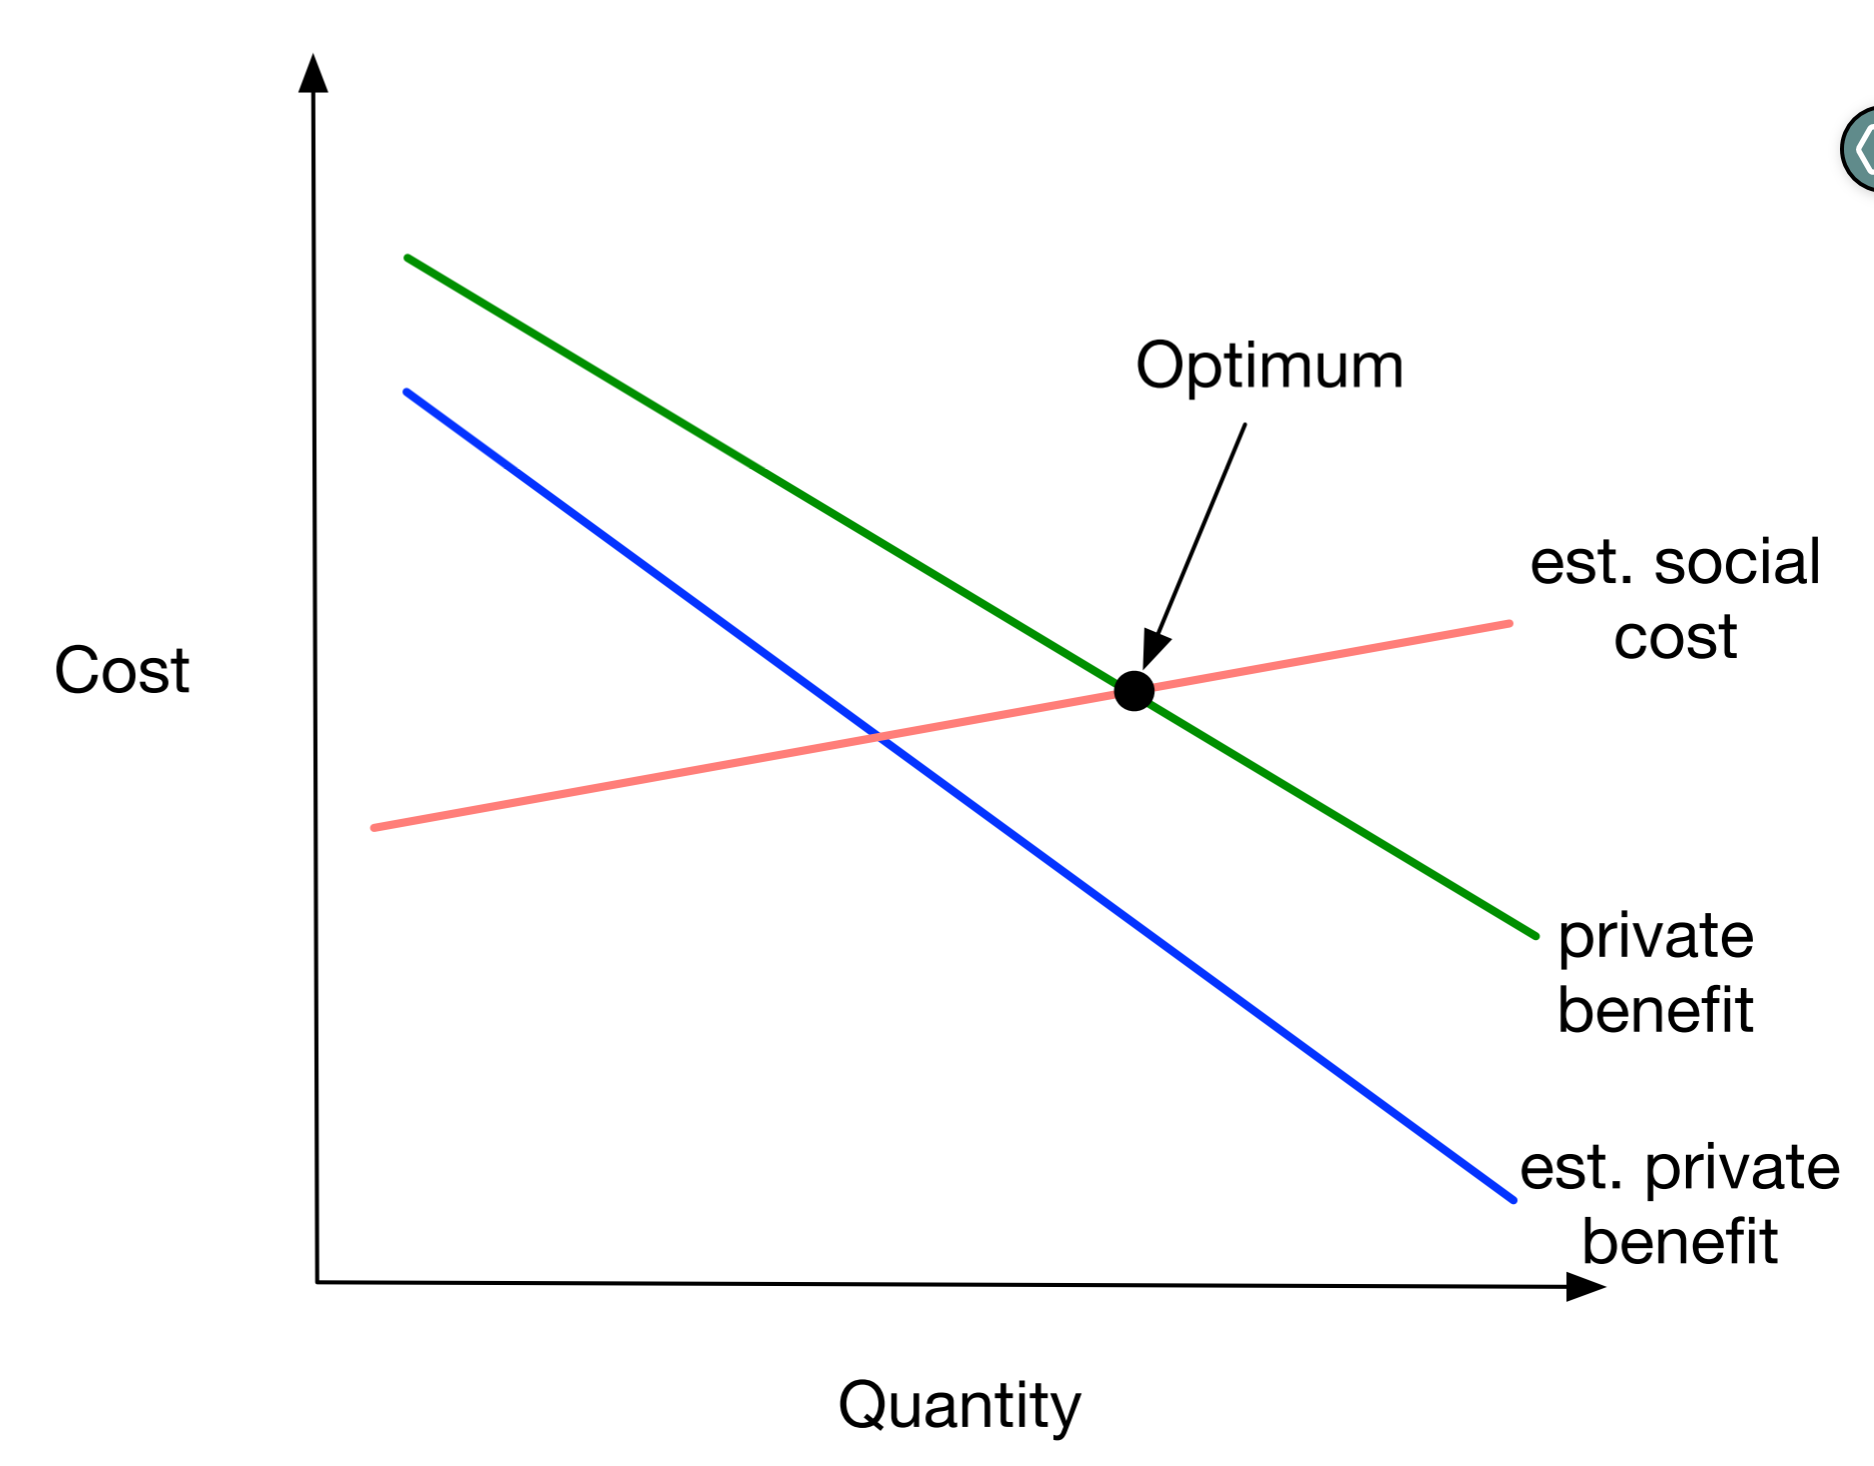
\includegraphics[width=2.25in]{fig1a.pdf}
%    \label{fig:1a}
%}
%\subfigure[]{
	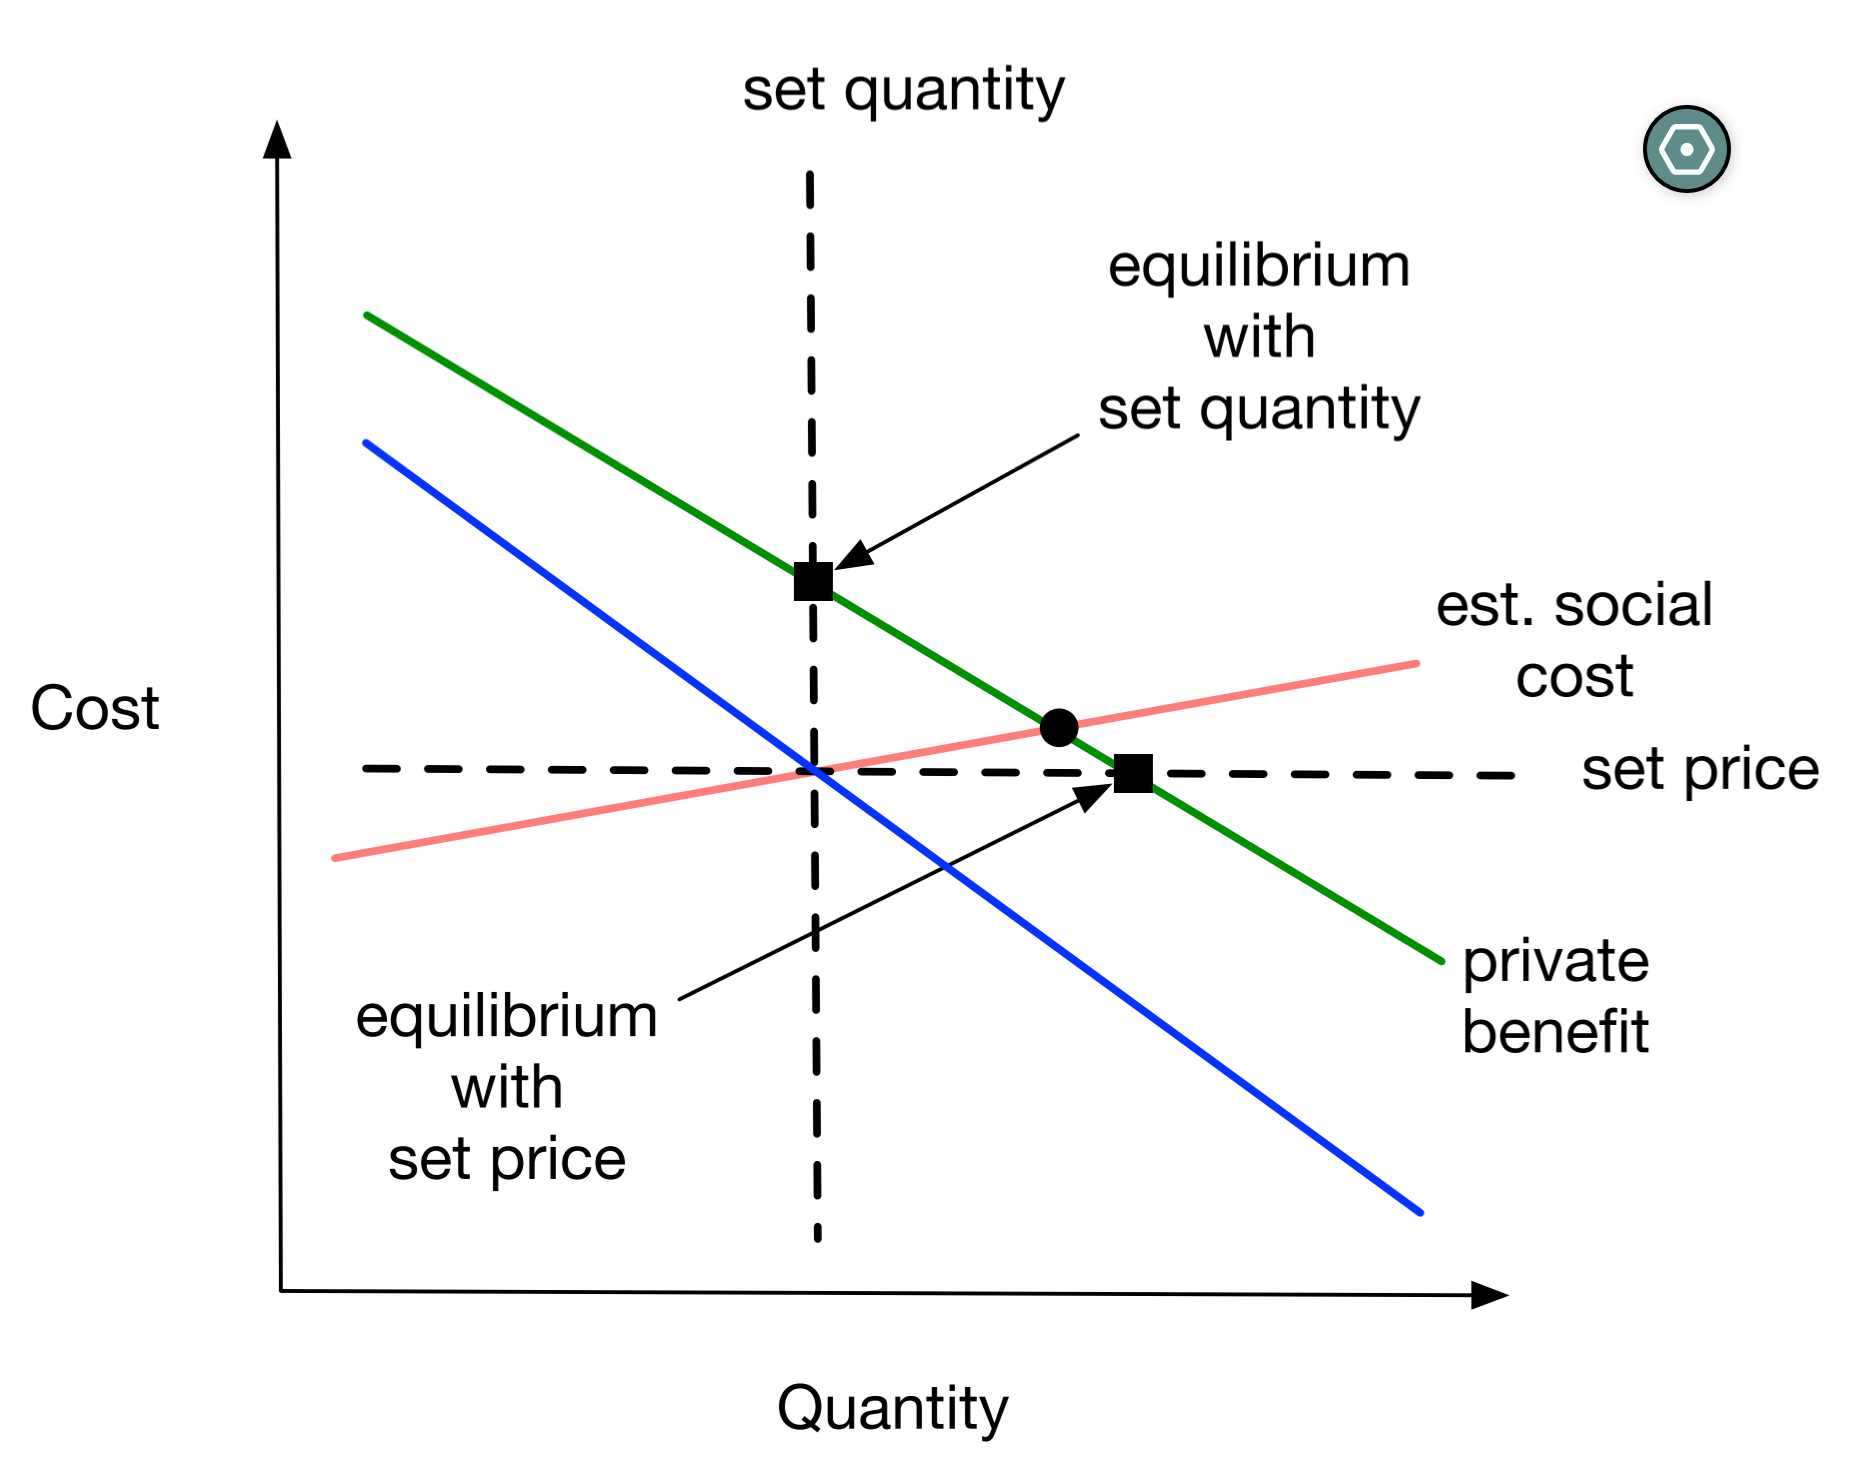
\includegraphics[width=2.25in]{fig1b.pdf} \\
%    \label{fig:1b}
%}

%\subfigure[]{
	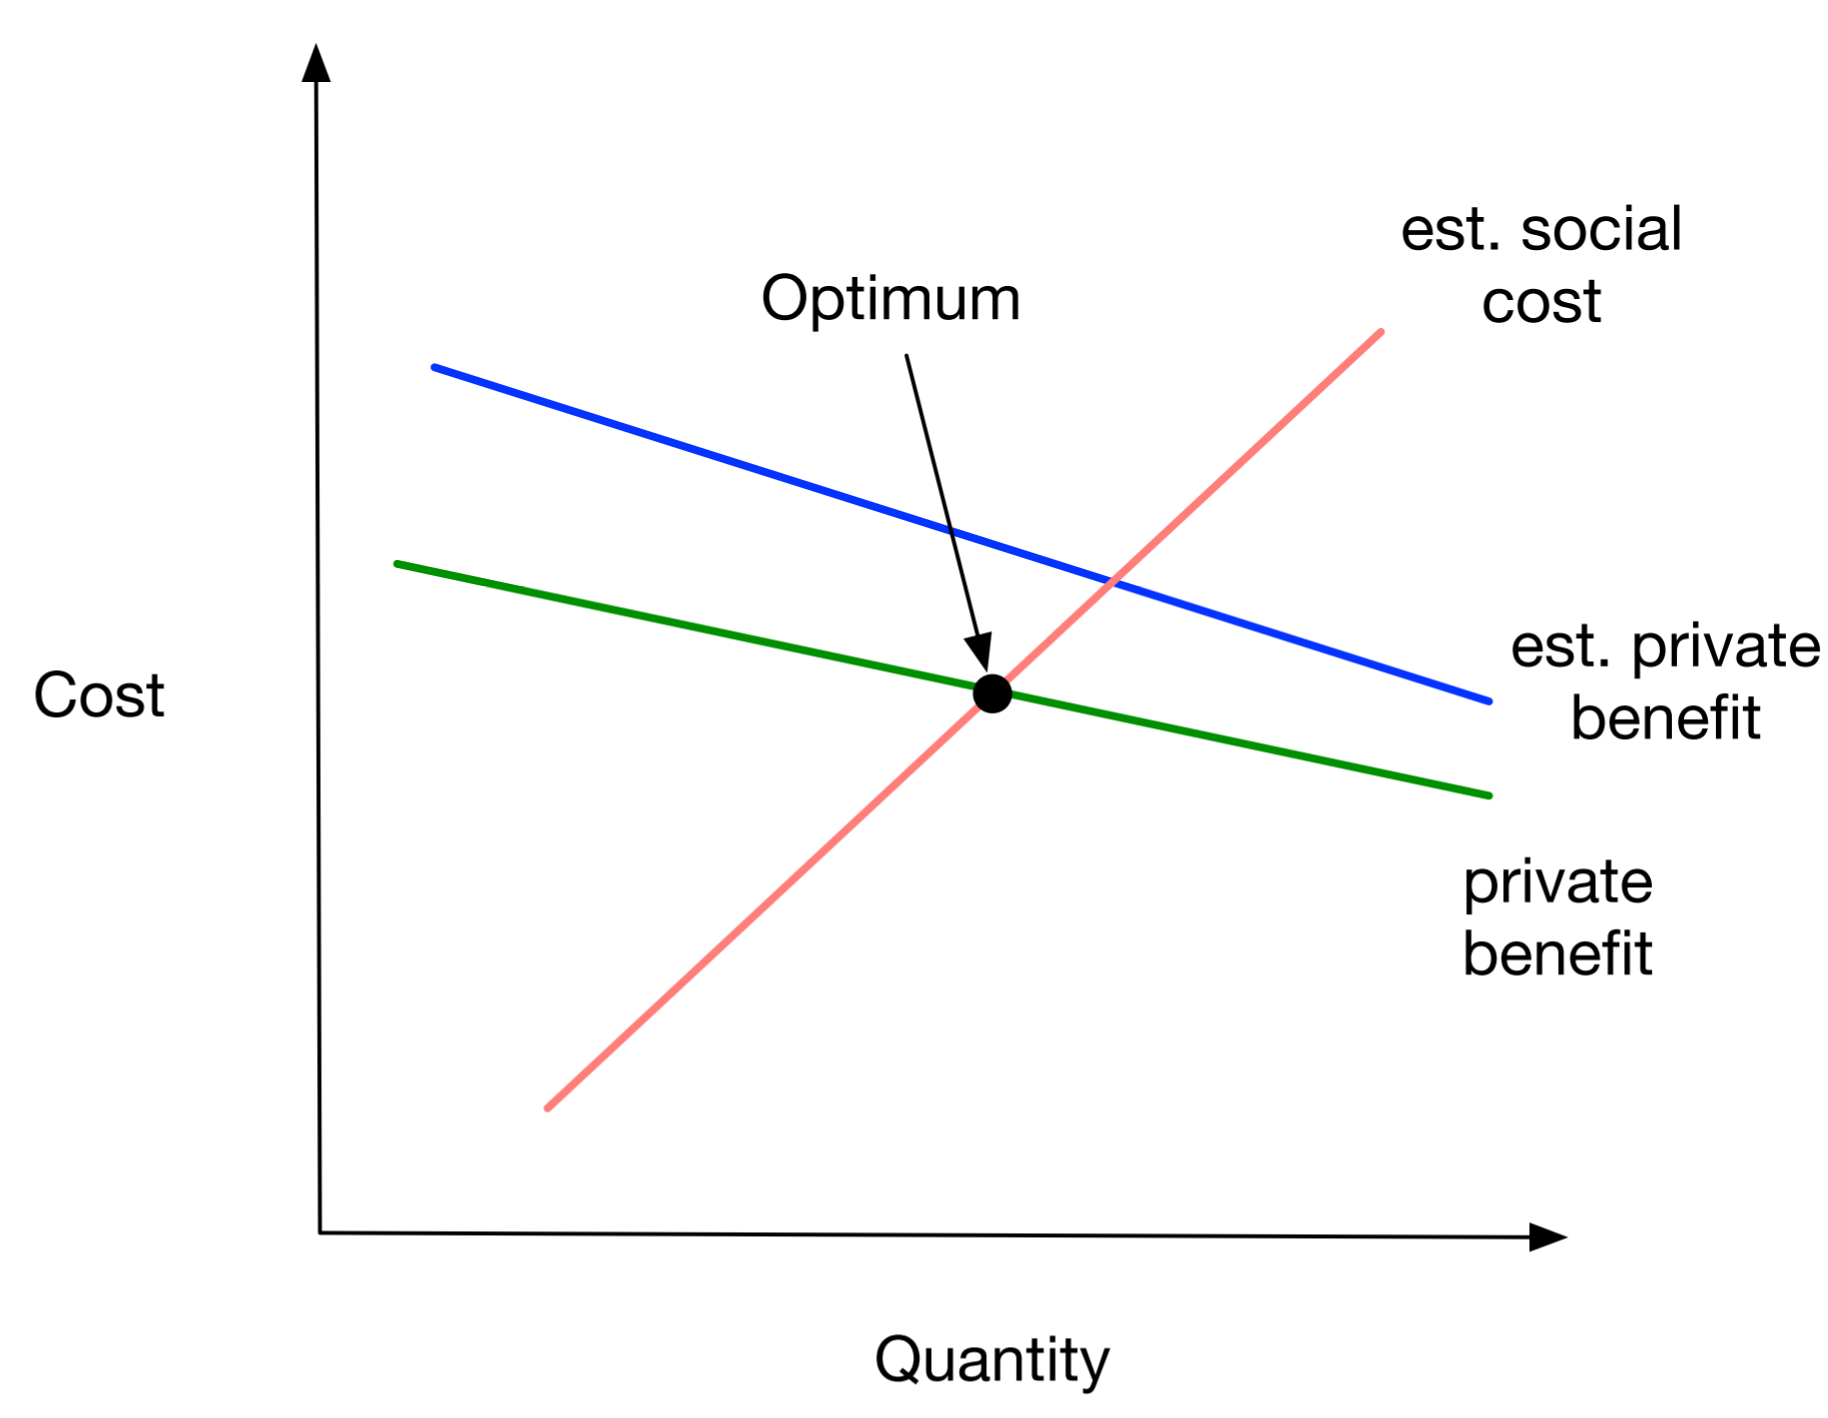
\includegraphics[width=2.25in]{fig1c.pdf}
%    \label{fig:1c}
%}
%\subfigure[]{
	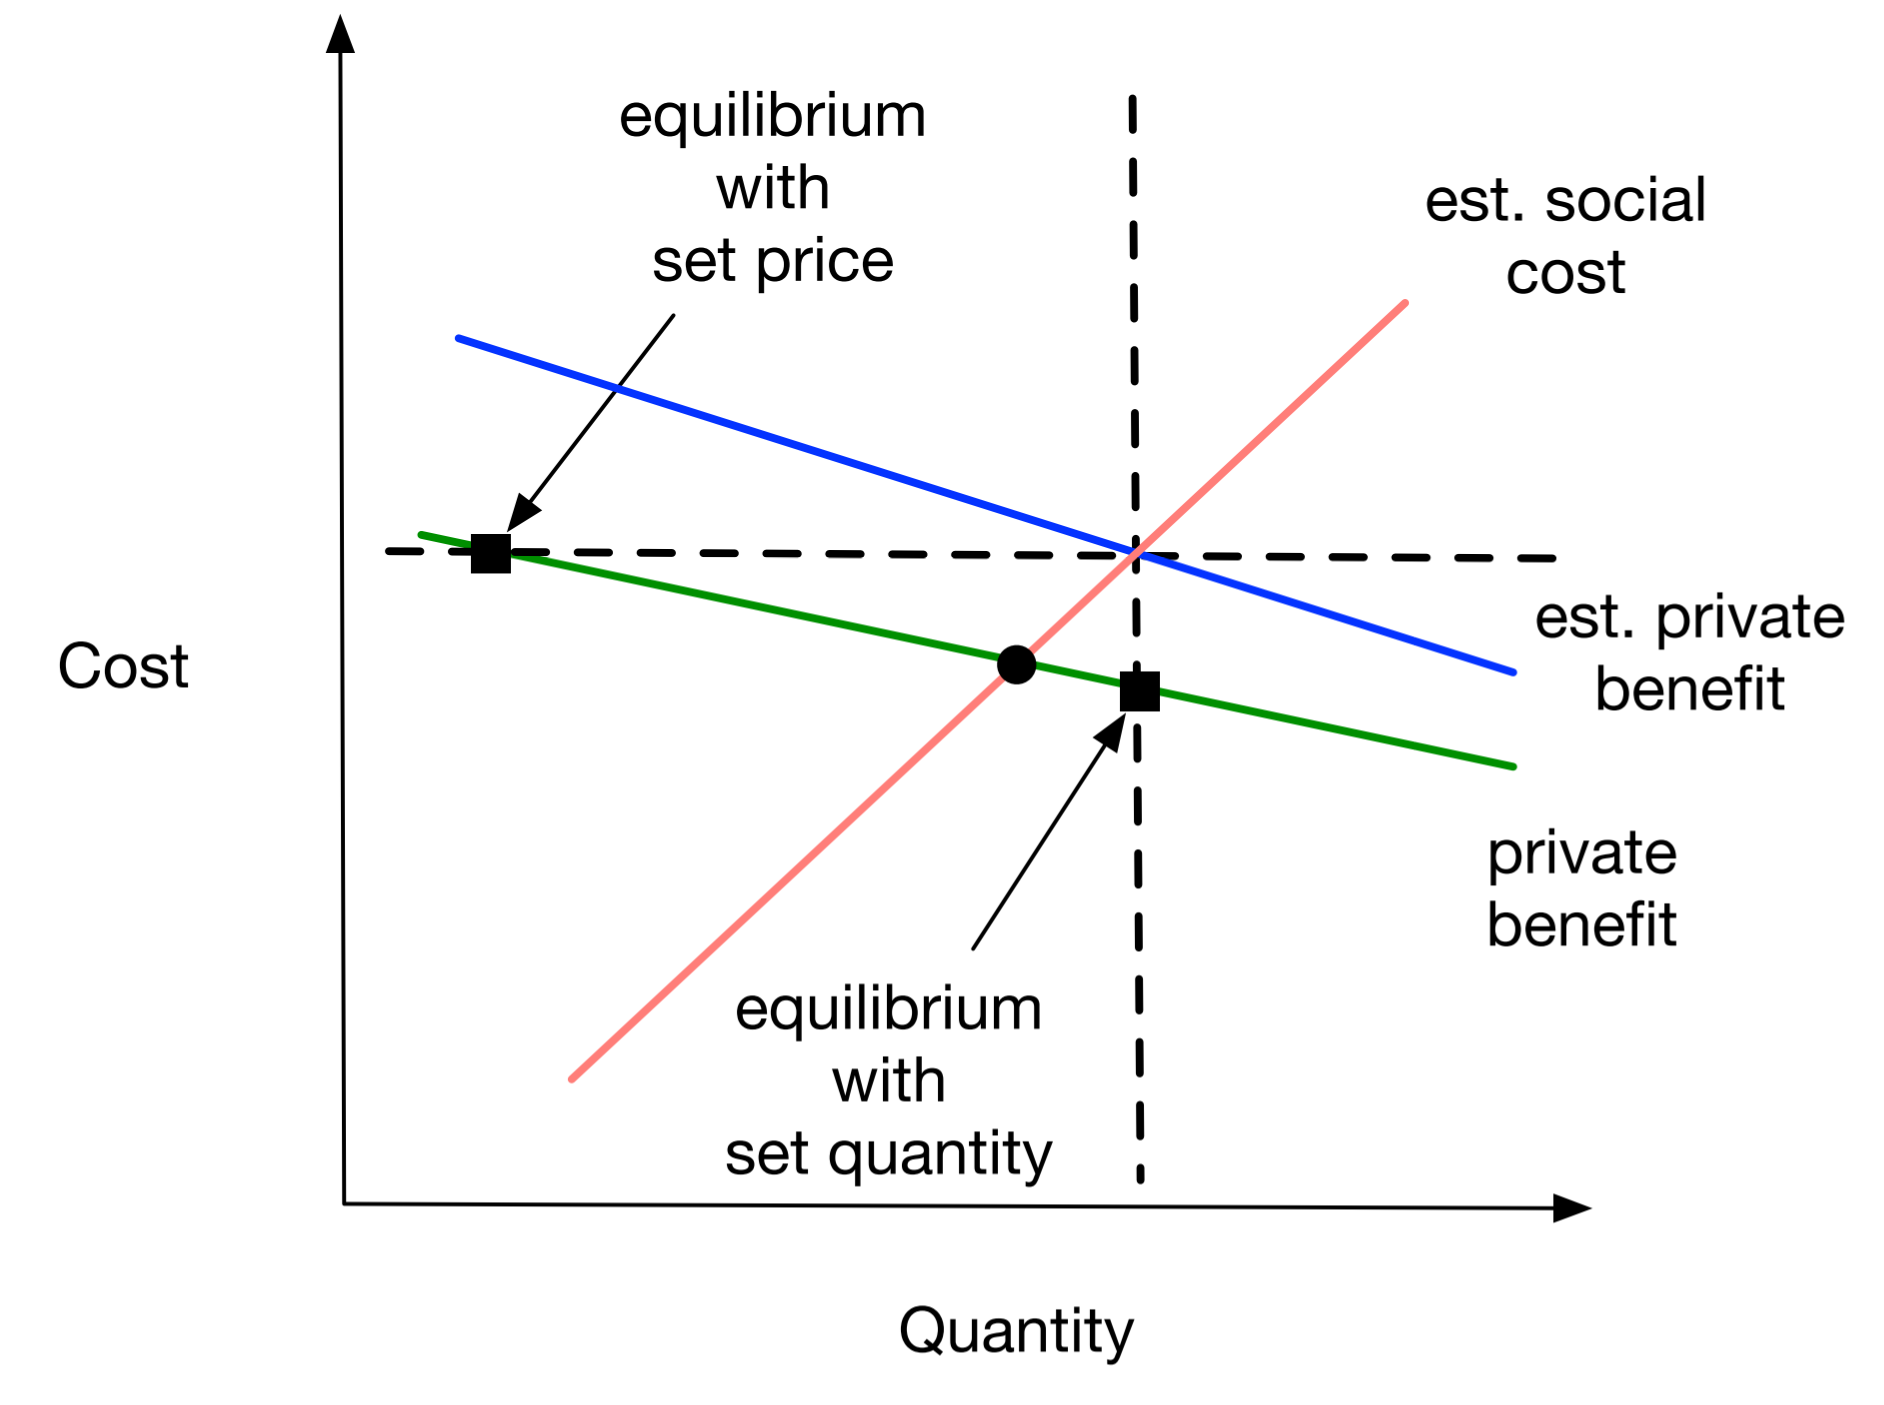
\includegraphics[width=2.25in]{fig1d.pdf} \\
%    \label{fig:1c}
%}
%\caption{Figures (a)--(b) show the first scenario in which it's better to set a price.  Figures (c)--(d) show the second scenario where it's better to set a quantity.}
Figures (a)--(b) show the first scenario in which it's better to set a price.  Figures (c)--(d) show the second scenario where it's better to set a quantity.
\label{fig:one}
\end{center}

Taken together, if the consumer's marginal private costs increase faster with quantity than the marginal social costs, then setting prices is better. But in the other case setting the quantity is better, or equivalently,

\begin{equation}
\frac{ \fname{cost\_to\_consumer}^{\prime \prime}( \opname{quantity} ) }{ \fname{cost\_to\_others}^{\prime \prime}( \opname{quantity}) }  > 1 \; ,
\end{equation}

then set prices.  Otherwise set quantity.  We use the second derivative because we are specifically talking about the \emph{the rate of change} in marginal costs.

The argument above applies only if costs and benefits are independently distributed. If changes in the cost and benefit curves are correlated, then an additional term must be added into the choice rule, increasing the relative attractiveness of limiting quantity. \new{To see this intuitively, consider the extreme case where uncertainty in cost and benefit is perfectly correlated; in such a scenario, if original estimates of cost and benefit prove incorrect, both curves will move up or down in lockstep, and so the new equilibrium will be directly above or below the original estimated one; hence, a quantity-targeting policy would be perfectly correct and a price-targeting policy would be pessimal.} This analysis covers only two possible policies, but a much greater space of options is available.  One can think of policy space as the space of possible supply curves for a given resource, where a pricing policy represents a horizontal supply curve and a cap-and-trade scheme represents a vertical supply curve. Various forms of diagonal supply curves are also possible, and in most cases some form of (possibly curved) diagonal supply curve is optimal.\footnote{ostrom2002}

Should blockchains have a block size limit, or should they not have a limit but instead charge a fixed fee per resource unit consumed, or would some intermediate policy, one which charges a fee as a function $F(w)$ of the weight included in a block and where $F'(w)$ is increasing and possibly reaches an asymptote, be optimal? To estimate optimal policy under the prices vs. quantities framework, we start off by attempting to estimate the social cost function.

A study from Cornell provided an estimate of the node count as a response to the weight load of the blockchain. The study was conducted at a time when Bitcoin's weight formula was simply one weight unit per byte, with a weight limit of $10^6$. The study found that 90\% of nodes would remain online at $W = 4*10^6$, and 50\% of nodes would stay online at $W = 3.8 * 10^7$.

%\begin{figure}
	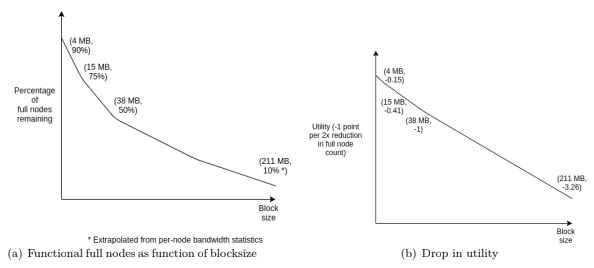
\includegraphics[width=5.5in]{blocksize_fullnodes.png}
%\end{figure}

%    \label{fig:1a}
    %\caption{Functional full nodes as function of blocksize from \cite{cornell-position}}

As a first approximation to quantifying the value to decentralization from having more nodes, we can use a logarithmic utility: $D(W) = log(NodeCount(W))$. What we discover is that $NodeCount(W)$ is roughly proportional to $\frac{1}{W}$, which in turn implies that $D(W) = -log(W)$. This in turn implies $D'(W) = \frac{1}{W}$: the marginal social cost function is \emph{decreasing}.

However, this model fails to take into account other kinds of harms that come as a result of large blocks taking a longer time to propagate. A study by Decker and Wattenhofer in 2013 found that the time that it takes for a block to propagate through the network is roughly linear in the block's size. Zohar and Sompolinsky\cite{GHOST} show that with a network delay $t$ and block time $T$, the rate of honest block creation slows from $\frac{1}{T}$ to $\frac{1}{T+t}$, reducing resistance to ``51\% attacks'' from $\frac{1}{2}$ to $q$ where $\frac{q}{1-q} * \frac{1}{T} = \frac{1}{T+t}$, i.e. $q = \frac{T}{2T + t}$. It seems reasonable to define a cost function $A(x) = \frac{1}{MinAttack(x)}$, where $MinAttack(x)$ is the minimum size of an attack that can succeed; since $MinAttack(x) = \frac{T}{2T + t}$, this implies that $A(x) = 2 + \frac{t}{T}$. $t$ is a function of $W$; if $t$ is linear in $W$, then that implies that $A(W) = 2 + k * W$ for some constant $k$, so the social cost function is linear.

In the case of Ethereum, we can try to look at the correlation between block gas usage and the ``uncle rate'', a measure of the percentage of blocks produced that do not make it into the canonical chain and hence that do not contribute to chain security.

\begin{center}
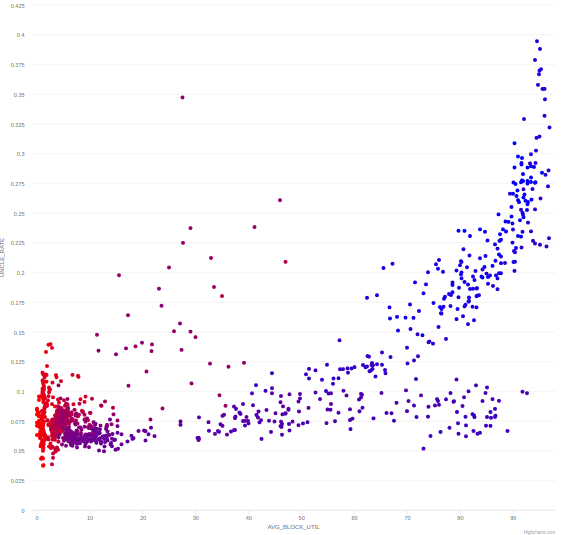
\includegraphics[width=3in]{etherchain_correlation.png} \\
Relationship between block gas limit and uncle rate
\label{fig:three}
\end{center}

The nonlinearity in this figure is in part an artefact of the data; during the period in late 2017, the composition of transactions changed away from smart contract use cases toward ERC20 token transfers, which affect uncle rate more than smart contract uses as their gas consumption is largely from bandwidth and computation costs and not code and storage. The dots at the top left are the 2016 DoS attack. Here's the same graph rescaled with the dots from late 2017 and the 2016 DoS attacks removed:

\begin{center}
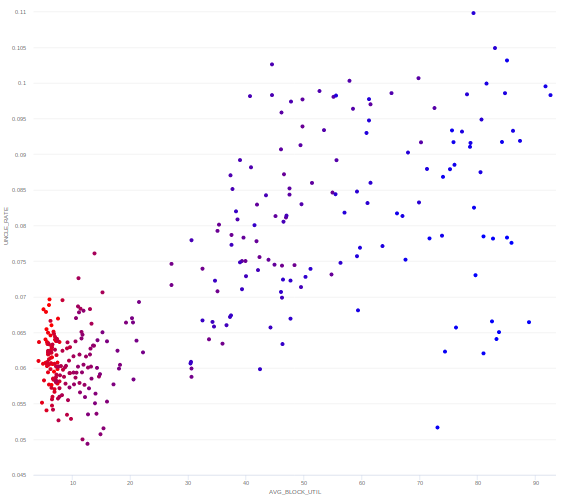
\includegraphics[width=3in]{etherchain_correlation_2.png} \\
Relationship between block gas limit and uncle rate, Dec 2016 to Sep 2017
\label{fig:three}
\end{center}

However, there are superlinear costs at play as well. Clients need to process both the main chain and the blocks that do not become part of the canonical chain; hence, if a level of canonical-chain throughput $x$ causes an uncle rate $p$, then the actual level of computational burden is $\frac{x}{1-p}$, with a denominator that keeps decreasing toward zero as the canonical-chain throughput increases. Additionally, with high uncle rates selfish mining attacks become much easier \todo{cite https://arxiv.org/pdf/1507.06183.pdf}, and the reduction in node count itself leads to pooling, which makes selfish mining more likely. There is thus a qualitative sense in which the social cost of $t = T$ is more than ten times that of $t = T * 0.1$.

Even if the cost function is superlinear at the extremes, however, it appears to be linear at the lower side of the distribution, and the arguments from the Cornell study suggesting it may even be sublinear. If the block size increases from 10kb to 1000kb, a significant social cost is incurred because IoT devices, smartphones, Raspberry Pis, etc have a much harder time staying connected, but an increase from 1000kb to 1990k does not have such a high cost, because the range of use cases that become unusable within that interval is much lower. Hence, it seems plausible that the social cost curve is U-shaped:

\begin{center}
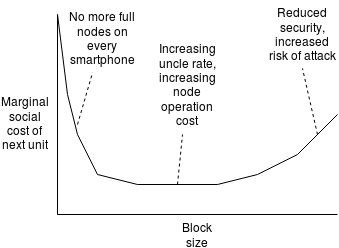
\includegraphics[width=3in]{total_social_cost.png} \\
Rendering of a possible total social cost curve for blockchains accepting transactions
\label{fig:three}
\end{center}

Note that there is a mixture of short run and long run effects at play here. A network can more easily adapt to transaction load increasing by a factor of ten over a year than it can to a similarly sized increase happening suddenly. If a Raspberry Pi can sync with the blockchain 98\% of the time, but suddenly fails to catch up 2\% of the time, then it may not be worth it to have the Raspberry Pi running at all. This suggests that the short-run social cost curve is more sharply upward-sloped than the long-run social cost curve; this is highly relevant when considering adjustable gas limits, "flex caps" and similar proposals.

\subsection{Estimating the Private Benefit Curve}

The private benefit curve, the demand for sending transactions, is much harder to estimate. We will try to make some estimates of a single variable, the elasticity of demand (ie. by what percent demand increases with a 1\% fall in price), by looking at some ``natural experiments'' in the Bitcoin and Ethereum blockchains.

One type of natural experiment is to look at day-by-day transaction fee changes during a situation where the capacity of a blockchain suddenly changes due to some extrinsic factor; Ethereum gas limit changes, and Bitcoin block time instability due to interaction effects between Bitcoin and Bitcoin Cash mining, are the easiest two cases. Charts show a correlation between reduced Bitcoin blockchain capacity due to temporary block time increases and transaction fee levels:

\begin{center}
%\begin{figure}[hbt]
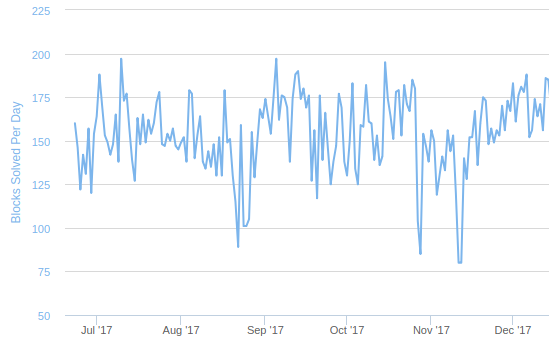
\includegraphics[width=2.5in]{bitcoin1.png} \\
Bitcoin blocks per day \\
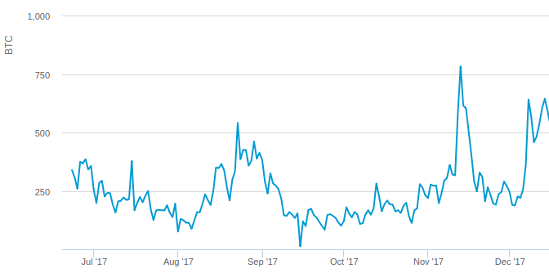
\includegraphics[width=2.5in]{bitcoin2.png} \\
Bitcoin transaction fees
\label{fig:three}
%\end{figure}
\end{center}

An more thorough analysis of similar data\cite{demand-elasticity} gives elasticities of 0.4-0.7 for Bitcoin, and 1-2 for Ethereum.

Additionally, it is important to note that this only measures the short-term demand curve looking at actions taken over a few days to months and does not take into account longer-term adjustments that could happen in the market only after a couple of years; in the real world, for example, it is an established fact that long-run demand elasticity of gasoline is higher than short-run elasticity\cite{env-econ}; and this is likely true with Bitcoin transaction fees and Ethereum gas as well.

So far, this model suggests a benefit curve with (rescaled) slope between -0.4 and -2, and a social cost curve with (rescaled) slope that is difficult to determine, but at current margins in various blockchains may be positive or negative. This suggests that a flat per-weight-unit in-protocol transaction fee, coupled with a hard limit at the point where the marginal social cost starts rapidly increasing, is superior to a pure weight limit-based regime.

------------------

\section{Cryptocurrency Prices}

In the short run, one can assume that price movements, changes in the social cost functions and changes in usage are all random and independent. In the long run, however, the three factors are highly intertwined. Specifically, (i) the price of a cryptocurrency; (ii) the social cost curve [as the number of beneficiaries of the system increases, and the number of full nodes also increases]; and (iii) the benefit curve [as there are more users sending transactions] are all highly correlated with a single variable, which we might call ``adoption''.

We can make a model as follows. Suppose that a k-factor increase in adoption leads to:

\begin{itemize}
    \item A k-factor increase in the price.
    \item A k-factor increase in the number of transaction users, ie. a k-factor horizontal stretch of the demand curve.
    \item A k-factor increase in the number of users and the number of full nodes.
\end{itemize}

Let us assume for simplicity that the demand elasticity is 1, and that the decentralization utility of $N$ full nodes is $D(N) = \log(N)$, so a k-factor increase in the number of full nodes simply adds utility $\log(k)$; the k-factor increase in the number of users scales up the social cost curve by a factor of k, and the private benefit curve scales by a factor of $k$. This leads to the result that, denominated in the cryptocurrency in question, adoption leaves the private benefit and social cost curves unchanged, and so there is also no correlation (!!). \footnote{An astute reader might ask whether or not empirical data supports this claim; unfortunately, far less than a single cryptocurrency ``business cycle'' (in the financial market bubble sense) has passed since blockchains started to typically have ``full blocks'', so there is far too little empirical data to make an assessment.}

Reality is of course more complicated than this simple model, but the model does suffice to show that, because of the lucky coincidence of being forced to denominate fees in a cryptocurrency whose price is itself proportional to adoption, there is at least no very strong first-order reason to expect positive correlation between the nominal benefit and cost curves. Hence, the arguments for using fixed fees in addition to gas limits still stand.

Arguably one of the key reasons behind the un-intuitiveness of fixed fees is that for most of the history of blockchain protocols, blockchains operated in a ``non-full blocks'' mode, where there was always space in a block to include more transactions. The fee required to be paid was only a minimal value, set as a software default. When a cryptocurrency experiences a large price rise, this causes fees experienced by users to rise greatly, until eventually the defaults are manually adjusted downwards \cite{coindesk-btc-txn-fee, reddit-rec-miners, vitalik-twitter1}.  Hence, transaction fees were kept artificially stable by what are essentially political factors, whereas no such stabilizing effect existed for cryptocurrency prices.

However, Bitcoin has recently entered the ``full blocks'' regime, where transactions are in permanent competition with each other to get included, and Ethereum has entered this regime during high-intensity token sales\cite{braveICO}. In this mode, fees become more volatile, and rises in adoption contribute to even more volatility. In Bitcoin, this has led to a $\sim 10x$ increase in fees in less than a year; in Ethereum, fees increase by a similar factor during token sales. Hence, it is now clear that, even under fixed quantity (i.e., fixed block size), fees can still be quite volatile even in the absence of price changes.

\section{Transaction Fees and Auction Theory}

So far, we have discussed resource pricing policies in the abstract, but we have not discussed the specific \emph{mechanism} that is used to implement them. The field of mechanism design has made many discoveries about what types of auctions perform better under what circumstances, and much of it is relevant to transaction fee markets.

In nearly all blockchains so far, transaction fee markets work as follows. Transaction senders are free to specify any fee they want as part of their transaction when they broadcast it. Transactions are included into blocks by \emph{block proposers}, which we can assume here are randomly selected for each block. Block proposers are constrained by the weight limit, which specifies how much they can include in each block. Naturally, block proposers will include the transactions that pay them the most, and as part of the protocol they collect the fees that are specified in the transaction.

In mechanism design speak, this is a \emph{first price auction}, characterized by the key property that ``you pay what you specify, and only if you win''. This kind of auction is generally considered to be deeply suboptimal, because it requires complex and inefficient strategies on the part of the buyers (here, transaction senders). For example, suppose that a given buyer values their transaction getting included at \$1. How much should they bid? The answer is certainly less than \$1; but how much less? If everyone else is bidding \$0.05, then clearly \$0.06 will suffice. If everyone else is bidding fees that have some complex distribution with mean \$0.10 and standard deviation \$0.05, with a fat tail on the right side, then the calculation becomes extremely complicated, and very often there are no efficient equilibria. \cite{poa-in-auctions} \footnote{The inefficiency of first price auctions in existing blockchain networks has already shown itself with many cases of users and businesses overpaying for fees \cite{bithumb-fees}, and self-help articles directing users to tools that facilitate ``fee estimation''\cite{fee-estimation}.}

The typical alternative is for selling many items a \emph{kth price auction}: everyone pays the same as the lowest fee that gets included. \footnote{Technically, everyone should pay the same as the highest fee that did \emph{not} get included, but this is even harder to implement and enforce, and for a sufficiently large number of items the difference between the two is very minor.} This mechanism allows for a very simple, and optimal, buyer-side strategy: if a transaction sender values getting their transaction included at \$x, they bid \$x. If the minimum bid in a block ends up being less than \$x, they get in (and pay less than \$x, so they are happy that they got in), but their bid being higher does not marginally affect the \emph{amount} they pay. If the minimum bid in a block ends up being more than \$x, the transaction sender does not get included, and is happy they were not included, because were they included they would have had to pay a fee higher than they were willing to pay.

However, kth price auctions have a different kind of serious flaw: they are not incentive-compatible \emph{for the auctioneer} (ie. the block proposer). First of all, if a block proposer is presented with a suitably steep demand curve, it is in their interest to fill the block with at least some high-fee-paying ``dummy transactions'', displacing low-fee-paying transactions and sacrificing the revenue from these transactions but at the same time dramatically raising the fee that \emph{everyone else} has to pay.

\begin{center}
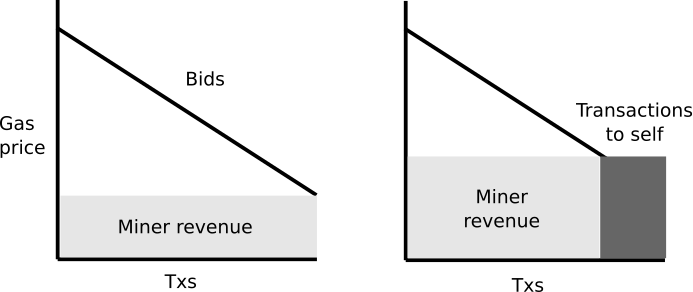
\includegraphics[width=3.5in]{kth_price_revenue.png} \\
\end{center}

A more serious issue is \emph{collusion} between the proposer and some transaction senders. A proposer can potentially collude with low-fee tansaction senders (eg. suppose there is a single entity, like an exchange or mining pool, that sends such transactions and can b easily negotiated with) that are sending transactions with some fee $f_{low}$. The proposer can ask them to instead send their transactions with fee $f_{high}$, and refund them $f_{high} - \frac{f_{low}}{2}$. The proposer's revenue is now even higher: the proposer benefits from the increased height of the ``rectangle'' of fee revenue that they would get with the ``dummy transaction'' strategy above, but they would also get a portion of the revenue from transactions that they would otherwise have sacrificed. \footnote{For a more detailed treatment of similar issues, see \cite{li2018} and \cite{rothkopf2007}.}

Hence, both first-price and second-price auctions are unsatisfactory. However, note that these issues are exclusively properties of auctions, and not properties of a fixed-price sale. If being included in the blockchain simply requires paying some $minFee$, then transaction senders have a simple strategy that they can use to set the fee on their transaction. Let $v$ be a user's private valuation for a transaction getting included in the next block. The user would check if $v > minFee$; if it is, they would bid $minFee + \epsilon$ (to provide a slight incentive for the block producer to include the transaction); if $v < minFee$ they would not send the transaction. This is a very simple strategy that does not require knowledge of others' valuations, and is optimal for the transaction sender.

\section{Improving the Second Best}

So far the evidence suggests that hard quantity limits are overused and price floors are underused. But how do we even start trying to set the price floor? What we will show in this section is that in cases where a price floor is better, it is possible to improve upon a hard quantity limit in a way that specifically alleviates the problem of deadweight losses from \emph{short-term transaction fee volatility}, without having to set a specific price as a protocol parameter. Clearly, large deadweight losses from short-term transaction fee volatility exist: Ethereum transaction fees are sometimes 2 gwei and sometimes 100 gwei, but it is definitely not true that the marginal social cost of a block containing 8000001 gwei rather than 8000000 is 50 times higher in the case where the latter is true.

Suppose that we start with an existing policy which sets a weight limit $w_{max}$. We normalize weight units so that the \emph{optimal} weight limit and transaction fee level are both 1. For simplicity, we assume linearity of the marginal social cost and demand function: $C'(1 + x) = 1 + C'' * x$ and $D'(1 + x) = 1 - D'' * x$, where $D''$ can also be viewed as the demand elasticity. Suppose that $w_{max}$ is set incorrectly, to $1 + r$ for some $r$ (in reality, $w_{max}$ will of course inevitably be set incorrectly, though we likely won't know the value of $r$ or even if it is positive or negative). We can draw a deadweight loss triangle to calculate the size of the economic inefficiency:

\begin{center}
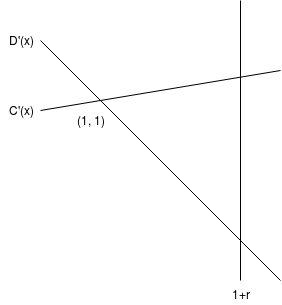
\includegraphics[width=2.5in]{Triangle1.png} \\
\end{center}

The area of the triangle, representing the total economic losses from an excessive (or if $r$ is negative, insufficient) number of transactions being included, is $\frac{1}{2} * r^2 * (C'' + D'')$; for simplicity we'll call this value $A$. Now suppose that, like in reality, demand is volatile, which we will approximate with a simple model where $D'(1 + x)$ half the time equals to $1 + D'' * x + \delta$ and the other half of the time equals to $1 + D'' * x - \delta$. In the $-\delta$ period, the height of the triangle increases from $r * (C'' + D'')$ to $r * (C'' + D'') + \delta$, or a ratio of $1 + \frac{\delta}{r * (C'' + D'')}$.

\begin{center}

\includegraphics[width=2.5in]{Triangle2.png} \\
\end{center}

By similar triangle laws the width increases by the same proportion, so the area increases from $A$ to $A * (1 + \frac{\delta}{r * (C'' + D'')})^2$. In the $+\delta$ period, the area decreases to $A * (1 - \frac{\delta}{r * (C'' + D'')})^2$. The average of $(1+x)^2 + (1-x)^2$ is $1 + x^2$, so the average of the two areas is $A * (1 + (\frac{\delta}{r * (C'' + D'')})^2)$.

Now, suppose we use a different algorithm. The protocol targets a \emph{long run} average weight of $1 + r$, but it does so by setting a price for transactions that adjusts slowly over time. The price that it would target is in this case is $1 - D'' * r$. Now, let us consider the average deadweight loss. Moving demand up by $\delta$ will move the triangle to the right by $\frac{\delta}{D''}$, which increases its height by $\frac{\delta * C''}{D''}$.

\begin{center}

\includegraphics[width=2.5in]{Triangle3.png} \\
\end{center}

The original height was $r * (C'' + D'')$, so the height increases by a ratio of $1 + \frac{\frac{\delta * C''}{D''}}{r * (C'' + D'')}$. By similar triangle laws the width increases by the same proportion, and in the $-\delta$ case we flip the sign in a similar way; the end result is that the average area is $A * (1 + (\frac{\frac{\delta * C''}{D''}}{r * (C'' + D'')})^2)$.

It should be clear that the average area in the second case is smaller (ie. less inefficiency) than the average area in the first case if and only if $\frac{\frac{\delta * C''}{D''}}{r * (C'' + D'')} < \frac{\delta}{r * (C'' + D'')}$, or alternatively $\frac{\delta * C''}{D''} < \delta$, or even more simply $C'' < D''$, and in other cases the average area in the second case is larger. What this thus proves is a sort of marginal analogue to Weitzman's 1974 result \cite{weitzman1974prices}, where in the exact same case where choosing a price is better than choosing a quantity, a quantity limit can be improved on the margin by replacing it with a ``flexible limit'' that is really just a price level that adjusts over the medium term to target the quantity limit.

We now propose an alternate resource pricing/limit rule that we believe provides superior properties to a hard limit $w_{max}$:

\begin{itemize}
\item Define a constantly adjusting in-protocol parameter $minFee$. Transaction senders are charged a fee of $minFee$ per weight unit; this fee is either burned or redistributed to consensus participants \emph{other than} the proposer of the block that included this transaction; this prevents profitable side-dealing arrangements where the transaction senders are refunded this fee.
\item Define a new weight limit, $w_{newmax} = 2 * w_{max}$.
\item Define an \emph{adjustment speed parameter} $adjSpeed$, with $0 < adjSpeed < 2$.
\item In any particular block, let $w_{prev}$ be the amount of weight consumed in the previous block, and $minFee_{prev}$ be the previous block's $minFee$ value. See $minFee$ for this block to equal $minFee_{prev} * (1 + (\frac{w_{prev}}{w_{newmax}} - \frac{1}{2}) * adjSpeed$.
\end{itemize}

This rule is likely to outperform simple limits in terms of allocative efficiency for the reasons cited above, and also (except during sudden and extreme spikes) eliminates the issues with first and second price auctions described above. \footnote{In the specific case of storage pricing, a quirk in Ethereum gas pricing rules that allows storage to be (mostly) paid for before it is actually used allows for second-layer markets like GasToken\cite{GasToken} where gas can be burned to generate ``congealed storage use privileges'', which can then be used later. The possibility of doing this unintentionally creates efficiency gains similar to those described here.}

As a philosophical note, complex gas and fee policies are often criticized as being a form of economic ``central planning'', which is frowned upon because planners may not have aligned incentives and have less information than participants closer to the day-to-day economic activity. That said, note that \emph{any} transaction pricing policy, whether fee-based or limit-based, necessarily has centrally planned parameters. I would argue that the correct way to apply the Hayekian anti-central-planning intuition is to treat it as saying that central plans are less bad if those plans have \emph{lower Kolmogorov complexity}, a simple strict weight limit being an ideal example.

Plans with low Kolmogorov complexity are ideal because they have fewer moving parts that can fail, are less likely to overfit, and because there is so little entropy in the specification and parametrization of the plan, it is very difficult to encode attempts to favor or disfavor specific users or applications; this helps foster a shared impression of fairness. For this reason, we will argue for policies that are as simple as possible while still being substantial and needed improvements on the status quo.

\section{Heterogenous Resources in Computation and Bandwidth}

The above weight limit analyses assume that a single scalar can sufficiently quantify the burden a transaction imposes upon the network. In reality, however, a transaction consumes several heterogeneous resources: calculation (Section \ref{sect:calculation}), state I/O (Section \ref{sect:io}), and state storage (Section \ref{sect:storage}).  Each of these have different properties, and an optimal pricing scheme should likely take these differences into account.

We will start off by looking at computation and bandwidth. Computation and bandwidth both contribute to the computational load of a node, and both contribute to ``uncle rate''; hence, both seem to be subject to the same mechanics of linear or sublinear social cost at lower weights and superlinear social cost at higher weights. If the factors creating the superlinear social costs are independent, it may be prudent to have a separate gas limit for computation and block size limit for bandwidth; however, because much of the superlinearity comes from the uncle rate itself, and the impacts of computation and bandwidth on uncle rate seem to be additive, it seems more likely that a single combined limit actually is optimal.

One question worth asking is: can we somehow measure in-protocol the amounts of computation and bandwidth




\section{Pricing Calculation}
\label{sect:calculation}
\todo{Calculation (e.g., arithmetic, comparisons, shuffling memory, hashing, verifying signatures) ...}

Pricing calcuation is the most straight forward.  Each transaction is executed by every full node.  So with $n$ full nodes, the cost of calcuation is $\Omega(n)$.  This is a one-time cost.

For example, between 1990--2005 computer clock speeds increased by $\sim \! 100$x \cite{40years}, but since 2005, growth in clock speeds has slowed down.  One interesting research direction is this: is it possible to somehow measure within the  blockchain protocol how fast clock speeds and seek times are \emph{right now}, and then automatically adjust costs to reflect these values?  For example, Bitcoin's difficulty adjustment is a rough proxy for calcuation speed.  Can Ethereum do something like this?  Failing that, are there general trends that can be used to ballpark predict how fast these improve over time?


\todo{add more about calculation here.}

\section{Pricing State I/O}
\label{sect:io}
State IO (i.e., reading and writing from the state) is unique because there are at least three ``modes'' of reading and writing to the state:

\begin{itemize}
\item If the entire is small enough to store in RAM, then reading is simply a memory-read, and writing is a memory-write together with an asynchronous process that copies the state modifications to disk.

\item If the state is too large to be stored in RAM, then reading requires reading from disk ($\sim\!100$ms on an SSD) and writing requires writing to disk. \question{It's unclear to me that these delays are quantifiable economic costs.}

\item If a light client wishes to fully verify a block, any state reads will be authenticated through Merkle proofs; each read or write will require at least $32 * \log(\tt{state\_size})$ bytes of proof data. \todo{cite}

\end{itemize}

Notice that there are now two distinct pricing strategies for state IO. One is to heavily restrict the total size of the state so that it will fit into RAM, and then charge cheaply for reading it (though writing should still be expensive, as it requires a disk write). The other is to let the state grow arbitrarily but charge as though a state read is always a disk read. Either strategy is legitimate.\footnote{However, keeping the state small has the ancillary benefit of light-client friendliness.  Encouraging blocks to be light on IO reduces both the number and burden of the Merkle proofs needed to prove validity.}

Between 1990--2005 hard disk seek times improved by a mer e$\sim \!\! 3$x \cite{ibm2011}, but with the advent of SSDs, reads/writes per second are increasing at an accelerating rate.






\section{Pricing State Storage}
\label{sect:storage}

Pricing state storage is a fundamentally different kind of burden from calculation and state-IO for one simple reason: whereas calculation are state-IO are one-time burdens on validators and nodes that are online at that particular time, but state space must be stored by, and thus burdens, all full nodes, forever. And for $m$ full nodes storing $n$ bytes the burden scales as $\Theta(m n)$ \question{true?}. The state is the data that a full node needs requires to validate a yet unknown subsequent block; in Bitcoin this is the ``UTXO set'', a representation of how many coins each user has, and in Ethereum this includes: account balances, contract storage, contract code, auxiliary information such as nonces, and the headers of the previous 256 blocks (as these can be accessed using the \opcode{blockhash} opcode).

More formally, accounts in each system can be viewed as a key-value mapping where each account is keyed by an ID number whose value is some balance in the system's base cryptocurrency (BTC/ETH) as well as other auxiliary data. In Bitcoin's case, the auxiliary data is constant (the scriptPubKey, a sliver of code describing the conditions for spending the balance). In Ethereum, contract accounts have their own storage, which is itself a key-value map whose contents may change over time.

In Bitcoin, this problem is not dealt with at all, and in fact Bitcoin's purely blocksize-based weight function is actively counterproductive: transactions that create many new UTXOs, and thus bloat the state, are cheap, but transactions that consume UTXOs, and thus clear the state, are more expensive, as each UTXO consumed requires an additional signature which nonnegligibly increases the transaction's weight. The segregated witness proposal mitigates this problem by reducing the cost of bytes in a signature by 4x, but the incentive misalignment remains.

In the case of Ethereum, there are two ways to increase storage size:

\begin{enumerate}
    \item The first is the \opcode{sstore} opcode, which saves a value in the contract's storage. If \opcode{sstore} overwrites an existing value, it costs 5000 gas, but if it adds a new value to storage, it costs 20,000 gas. If \opcode{sstore} is used to clear an existing value (so it no longer has to be saved in the trie), then it costs the contract 5,000 gas, but a ``refund'' of 15,000 gas is given to the transaction sender.

    \item The second is \emph{account creation}. Accounts can be created\footnote{Accounts can also be deleted through the \opcode{selfdestruct} opcode, which costs the contract 5,000 gas but refunds the transaction sender a 24,000 gas.} in three ways:

    \begin{itemize}
        \item creating a contract using the \opcode{create} opcode (32,000 gas, plus 200 per byte of code)
        \item creating a contract using a transaction (53,000 gas, or 32,000 + the 21,000 base cost of sending a transaction)
        \item sending ether to a previously non-existent account (25,000 gas if done from a contract; if done from a transaction the 21,000 gas base cost).

    \end{itemize}

\end{enumerate}


One simple solution is to increase the costs for permanent storage by making an across-the-board recalculation of storage-filling opcodes and refunds based on a 500--1000 cost per byte. This could be done in combination with a gas limit increase in order to make the change neutral with respect to average transaction capacity. However, even with such a change several challenges remain.

\begin{itemize}
\item There is insufficient incentive to clear storage. Although there are refunds when using \opcode{sstore} and \opcode{selfdestruct}, they are small refunds.  Increasing the refunds is risky, because it opens the door to arbitrage. For example, under full-block volatile-gas-price conditions, users could fill storage during the weekend when gas prices are low and then get refunds at peak time when gas prices are high.  Furthermore, refunds can only make future transactions cheaper, not give money back.

\item There is no monetary incentive to clear storage now instead of fifty years from now---the size of the refund is the same regardless of when you do it.

\item Even when blocks are not full, validators still have a disincentive against including blocks: the larger and more computationally intensive the blocks are that they create, the longer they will take to propagate through the network, and so the larger the chance they will not be part of the main chain, leading to losses of rewards for the validator.

Etherchain runs linear regressions to compute the average implied cost \cite{etherchaingas} to a validator of adding each unit of gas to zer blocks, and currently it is $\sim \!\!0.013$ ETH per million gas. However, if a gas-intensive transaction is paying primarily for storage rather than computation (e.g., as in contract-creating transactions), the gas represents long-term storage costs and not costs to present-day computation, and so for those transactions this risk does not exist. This incentivizes validators to favor storage-filling transactions, and makes the optimal validator strategy much more complex, possibly favoring the emergence of centralized pools that optimize their blocks through private agreements with application developers.

\item When blocks are not full, validators have the ability to ``grief'' the network by sending transactions to the network that increase the state size at no personal cost.

\end{itemize}

Suppose that for the reasons above we do not implement in-protocol rent, and instead only allow users to purchase storage at a high price (e.g., using the first proposal above to greatly increase the gas cost). Then, there may be users who create contracts with a large number of storage slots, and ``rent them out'' - anyone can ask the contract to rent out a batch of storage slots for some fee, and for some time they will be given permission to read and write to those slots. Provided the ratio between the cost of filling new storage and the cost of editing existing storage is high enough, there will invariably be an incentive to do this, and this may satisfy many of the goals of in-protocol rent markets.

\todo{We need to come down on one side of the rent issue.  Do we support it or not?}

\subsection{Implementing Rent}


One popular proposal is ``storage rent''. The idea is simple: every account object is charged X coins per block per byte that it consumes in the state. If an account has less coins than the amount needed to pay for $N$ blocks (say, $N = 500$), then anyone can ``poke'' the account and delete it from storage, and claim $k N$ blocks' worth of rent as a bounty where $k \in (0,1]$. Implementing the above is impractical as every block going through every account and decrementing its balance has immense overhead. However, this is a better way, and we propose the following scheme:

All accounts store an additional data field, last\_block\_accessed. In the case of Ethereum accounts, another data field, storage\_slot\_count, is added to denote the total number of storage slots in each account.

We define an extending sequence $\opname{crf} = (0, x_1, x_2, \ldots )$ where $x_i = x_{i-1} + \fname{rent}(i)$, where function $\fname{rent}$ takes a block index $i$ and returns a nonnegative integer fee for storage during that block, and may be computed by an arbitrary formula. Using this mechanism, {\tt{crf}} stores a ``running sum'' for the total rent fee, and $\opname{crf}[j] - \opname{crf}[i]$ computes the rent per byte to be paid from block $i$ to $j$.

When any account is touched, update via Algorithm \ref{alg:storage_update}.

% asize = account's current size in bytes\;
% abalance = account's current balance\;


\begin{lstlisting}
 \KwData{block\_number, acct, caller\_id, size\_delta, crf}
 \KwResult{Adjust account's total size}
 current\_crf = $\opname{crf}$[block\_number]\;
 {\tt{acct.balance}} $-$= {\tt{acct.size}} * ($\textnormal{current\_crf} - \opname{crf}[{\tt{acct.block\_last\_accessed}}$)\;
 \ 
 \eIf{ {\tt{acct.balance}} $< 500\ * (\textnormal{current\_crf}\ -$ $\opname{crf}[\textnormal{block\_number} - 1])$ }{
 transfer( {\tt{acct.balance}}, caller\_id )\;
 {\tt{acct.self\_destruct()}}\;
 }{
 {\tt{acct.last\_block\_accessed}} = block\_number\;
 {\tt{acct.size}} += size\_delta\;
 }
 \caption{Algorithm to update the storage size.}
\label{alg:storage_update}
\end{lstlisting}



The rent scheme in Algorithm \ref{alg:storage_update} adds a strong incentive to: not consume a large amount of storage as well as minimize storage time (clear early).  We require that storage rent costs are not given to validators.  This is to ensure validators are never incentivized to ``bloat'' the state or even seek storage-filling-heavy transactions.  This rent solution resolves all known incentive incompatibilities in storage pricing (Section \ref{sect:storage}). However, it damages developer experience by:

\begin{itemize}
\item the fundamental guarantee that once something is in the state, it stays in the state, is now gone.  Developers now have to become economists, coming up with pricing schemes to charge for access to these systems so that they can pay for their ongoing rent to ensure the contracts' continued existence. 

\item Applications that interact with applications have to check that not only their application, but also every application that their application depends on, and so on recursively, stays alive.
\end{itemize}


One modification to rent to improve developer experience is exponential ``rent-to-own'' storage pricing.  This scheme can be described as follows. Every time an account increases its size (a newly created account is viewed as increasing its size from zero), it pays a fee of ${\tt{storage\_price}} * (\textnormal{new\_account\_size} - \textnormal{old\_account\_size})$, denominated in the base cryptocurrency. This fee is added to the account's ``deposit'' (a kind of secondary balance). Every block,\footnote{Just as in the previous scheme, it is vastly more efficient to calculate the decay just-in-time.} every account's deposit is multiplied by, $1 - \frac{1}{\tt{ACCOUNT\_DEPOSIT\_DECAY\_FACTOR}}$.  When an account decreases its size (an account being deleted can be viewed as decreasing its size to zero), it receives a refund of,
\begin{equation}
\textnormal{current\_account\_deposit} * \frac{\textnormal{old\_account\_size} - \textnormal{new\_account\_size}}{\textnormal{old\_account\_size}},
\end{equation}
 and this amount is removed from the account's deposit.
 
This scheme weakens the ``neutrality'' of storage pricing, but it improves developer experience by making storage cheaper if an account has already held it for a long time.  We deem this an acceptable trade-off.  \question{Wouldn't this encourage rent-database contracts even more?}

\todo{Have moved Dapp resurrection to the Appendix until we have a protocol for handling multiple resurrections.}

\subsection{Paying for storage in a new internal currency?}

The above schemes also expose another dichotomy: should storage be paid in gas (or, more generally, the ``weight'' metric of a blockchain), or be paid in the base cryptocurrency?

There are two primary arguments for charging for storage in gas:
\begin{itemize}
\item \textbf{Simplicity}. Simplicity is a virtue. The protocol is simpler when there is only one mechanism for charging for resource consumption.
\item \textbf{Less overhead} When accounts constantly consume a protocol's base cryptocurrency, additional transactions are required to keep accounts ``topped up''.
\end{itemize}

Note that, unlike Bitcoin's UTXO-based systems where account objects are created once and destroyed once, less overhead applies much more strongly to Ethereum, where accounts can have complex internal states and persist over the course of many interactions.

There are several primary arguments for charging in a protocol's base cryptocurrency, or even defining an additional in-protocol resource.

\begin{enumerate}
\item \textbf{State space price stability}.  Decoupling pricing of state space consumption from a volatile transaction fee market makes state space pricing more stable, and allows for the design of a special-purpose fee schedule and supply curve that further promotes stability. This has two benefits:

\begin{itemize}
\item \textbf{Economic optimality}. Economic analysis dictates that state space prices should be stable in the medium term due to the social cost of state space consumption does not change quickly.

\item \textbf{Reducing attack surface}. Attackers have vastly more means to influence gas prices.  If storage prices were in gas, and an attacker can quickly devalue gas, then ze can interfere with applications by causing objects to get deleted much earlier than their developers thought.
\end{itemize}

\item \textbf{Clean separation}. Freedom to design a separate supply curves for state space consumption and calculation/state-IO.

\end{enumerate}

Furthermore, in the specific case where rent is charged per-block, the fees paid by account objects during some block are not in any significant sense tied to transactions within that block, and so charging transaction senders is not a very natural solution.

If fees are paid in a protocol's base cryptocurrency, then another question appears: how much to charge? Should there be a fixed price, should the price adjust up and down to target some rate of state size growth, or something in between? This is still arguably an unsolved research question.



\section{The Two-currency Solution}
\todo{We talk about how to merge the measures from Sections 4--6 into a one or two dimensional gas measure.}
\todo{Come down on one side of whether want a new internal currency just for storage.}

\section{Conclusion}

\todo{fill in conclusion here.}

\textbf{Future work.} \todo{fill me in.}

\textbf{Acknowledgements.} \todo{fill me in.}


\bibliography{ethpricing}


\newpage
\appendix
\part*{Appendix}

\section{Unused text}

\todo{This is text that was in the paper but has moved here until a home has been found for it. If no home is found will delete.}


A more a-priori mathematical model might assume that the bandwidth of full nodes is power-law-distributed; if this is true, then an m-factor increase in the block size would decrease the number of full nodes by a factor of $n$; that is, an m-factor increase in the block size would cause a constant loss of utility, and so the marginal social cost of an additional transaction is proportional to the inverse of the existing load of the chain. We suspect that there are fundamental limits to the capacity of a node because of limits to clock speed and Amdahl's law [cite], though even in the chart above we see the marginal social cost of an additional transaction very slightly decreasing. 


Fourth, proof of work blockchains present the possibility of using mining difficult as a (very rough) proxy for price; unfortunately, in a proof of stake blockchain even this is not possible.  One possiblity is requiring some kind of non-outsourceable memory-hard proof-of-work for transaction sending, and using this to estimate the computational resources available to users.  But this is potentially very fragile.


These gas costs are calculated based on a formula that assigns a 200 gas cost to each byte saved in storage. An \opcode{sstore} is deemed to consume $\sim\!75$ bytes because it stores a 32 byte key and a 32 byte value, with an additional 11 byte overhead for the intermediate Merkle tree nodes (likely an underestimate). An account is deemed to consume $\sim\!128$ bytes: 3 for a nonce, 8 for a value, 32 for a code hash, 32 for a storage trie root hash, 20 for the account address, 5 for serialization overhead and $\sim\!28$ for state tree overhead (also possibly an underestimate). 

Even ignoring gas arbitrage, there remains a serious incentive incompatibility arising from the fact that, whereas the average price should presumably be more expensive in periods of high congestion, storage price should be stable over the medium term, a goal at odds with the inherent volatility of gas prices in full-blocks conditions. \question{Shouldn't this apply to Calcuation and IO as well?}

\textbf{Calculation and Custom Optimization}

Another discrepancy is that between different types of computation, and specifically the possibility of optimization (both software, through custom implementations, and hardware, through FPGAs and ASICs). Even though Ethereum runs on a general-purpose virtual machine, at least the overhead of the VM is too high to run intensive cryptographic operations within it; for example, implementing cryptographically anonymized voting led to a system where a single transaction took up half an Ethereum block. \cite{fc17ai}

Even ignoring VM overhead, many cryptographic operations are hardware optimized, and due to the seemingly inescapable very high overhead for new forms of cryptography such as zk-SNARKs, homomorphic encryption, and indistinguishability obfuscation, it seems inevitable that hardware optimizations will be done for those too. A blockchain protocol with a general-purpose virtual machine could always simply add special-purpose ``opcodes'' (or ``precompiles'') for such optimized operations, assigning them a weight that reflects their runtime with the hardware optimizations. But we'’d prefer to detect such optimizations automatically, incentivizing validators to voluntarily agree to reduce weights for operations that they can compute efficiently. However, there are a number of serious complications for such a scheme. First, how will the scheme deal with situations where 60\% of validators have an optimization but the remaining 40\% don't? If the scheme attempts to target 90\% support, then what happens if 11\% attackers stall the system by pretending not to have a given optimization? What happens if an attacker creates an operation which is normally slow to execute, but the attacker has a ``trapdoor'' that allows them to execute it quickly (any digital signature scheme can be easily turned into such a scheme), and then pretends this is a special operation for which the attacker has an optimization?


\subsubsection{Dapp resurrection}

Accounts that run out of ether to pay rent can get deleted, but anyone can always submit a Merkle proof that a contract previously existed at some address and thereby resurrect it. This resurrection keeps total neutrality of storage pricing, but has two major flaws:

\begin{itemize}
\item Contracts must account for the possibility that contracts may be \emph{temporarily unavailable} or ``hibernate''. 
If a contract hibernates with state A, then is resurrected, then hibernates again with state B, then one can form a valid proof to resurrect it with A or with B, and an interactive game would be required to detect the more recent resurrection. Doing this correctly is an unsolved problem, and furthermore any solution would increase the complexity to the protocol and security model.

\item Note that in both the original scheme and these two modified schemes, there remains a problem of calculating exactly what the storage price should be.
\end{itemize}

---


\textbf{No costless griefing}. Even when blocks are not full, validators should not be able to permanently consume storage for free.



%%%%%%%%%%%%%%%%%%%%%%%%%%%%%%%%%%%%%%%%%%%%%%%%%%%%%%%%%%%%%%%%%%%%%%%%%%%%%%%%%%%%%%%%%%%%%%
%% TABLES!
%%%%%%%%%%%%%%%%%%%%%%%%%%%%%%%%%%%%%%%%%%%%%%%%%%%%%%%%%%%%%%%%%%%%%%%%%%%%%%%%%%%%%%%%%%%%%%



%\begin{figure}
%\centering
%\subcaptionbox{Subcaption A}{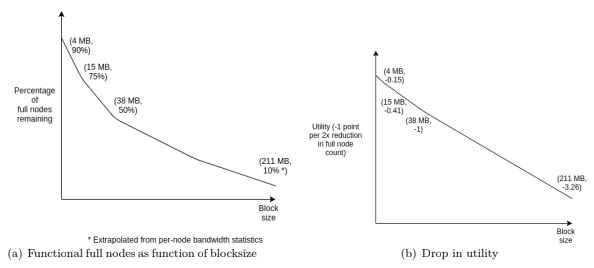
\includegraphics[width=3in]{blocksize_fullnodes.png} }%
%\hfill
%\subcaptionbox{Subcaption B}{ 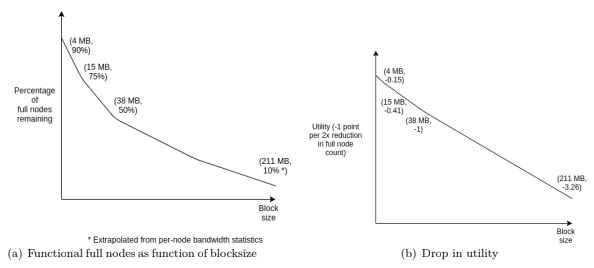
\includegraphics[width=3in]{blocksize_fullnodes.png} }%
%\caption{Caption}
%\end{figure}




\section{The Full Ethereum Gas Function}
\label{appendix:gasfunction}
\todo{Put the full gas function here.}


\end{document}
  
  
  
  
         

        
